\section{Prompt Templates}
\subsection{Bi-Arm Bandit Environment Prompts}
The Bi-Arm bandit environment implements a classic reinforcement learning problem where an agent must balance exploration and exploitation. We present the prompt templates below.
\begin{tcolorbox}[colback=gray!2, colframe=black, boxrule=0.5pt, arc=2pt, width=0.95\linewidth, title=Model Templates]

\texttt{<|im\_start|>[system]:\\
\{prompt\}\\
You're a helpful assistant. You always respond by giving your answer in <answer>...</answer>. Max response length: 200 words (tokens).\\
<|im\_end|>\\
<|im\_start|>[user]:\\
\{prompt\}\\
You are playing a bandit game. Goal: Maximize your total reward by choosing which arm to pull. \\
Game Rules: \\
1. There are 2 arms, named {name\_a} and {name\_b}\\
2. Each arm has its own reward distribution, related to their names. \\
3. Analyze the symbolic meaning of each arm's name to guess how their reward distribution might behave.\\
4. Based on the symbolic meaning of their names, which arm do you think is more likely to give higher rewards on average? Choose between {name\_a} and {name\_b}, and output like <answer> {name\_a} </answer> or <answer> {name\_b} </answer>.\\
<|im\_end|>\\
<|im\_start|>assistant\\
<think>}

\end{tcolorbox}
% The environment uses two numbers to represent different options:

% \begin{promptbox}{Environment Representation}
% \texttt{State:\\
% Machines: Trader(1), Librarian(2). Choose: [1, 2]\\
% You have * actions left
% }
% \end{promptbox}
% To introduce the task to the language model, we provide a comprehensive guide that explains the game mechanics, rules, and expected action format:

% Task Introduction
% \begin{promptbox}{Task Introduction}
% You are playing a multi-armed bandit game.

% \textbf{Multi-Armed Bandit Quick Guide}\\
% Goal: Maximize your total reward by choosing which arm to pull.

% \textbf{Game Rules:}
%     1. There are $n$ slot machines (arms), numbered 1-$n$\\
%     2. Each machine has its own reward distribution\\
%     3. Rewards are drawn from a normal distribution\\
%     4. The mean reward for each machine is fixed but unknown\\
% \textbf{Actions:}\\
% Choose a number between 1 and $n$ to pull that arm\\
% Format: \texttt{<answer> [number] </answer>}

% \textbf{Strategy Tips:}\\
%   - Balance exploration (trying different arms) and exploitation (using arms known to be good) \\
%   - Keep track of the rewards you receive from each arm
% \end{promptbox}

% The instruction template combines the task introduction with the current state observation to form the complete prompt:

% % Instruction Format
% \begin{promptbox}{Instruction Template}
% \texttt{\{task\_intro\}\\}
% \texttt{[Current State]:\\}
% \texttt{\{observation\}\\}
% \texttt{Choose which arm to pull:}
% \end{promptbox}

% For state representation, we implement two different rendering formats depending on whether it's the initial state or a subsequent state after an action:

% % Observation Rendering
% \begin{promptbox}{State Rendering}
% \textbf{Initial State:}\\
% \texttt{You are facing $n$ slot machines (numbered $k$ to $k+n-1$). Each machine has its own reward distribution.\\
% Which machine will you pull?}

% \textbf{After Action:}\\
% \texttt{You pulled machine $m$.\\
% Which machine will you pull next?}
% \end{promptbox}

% Finally, we provide feedback to the model about the validity of its actions and the resulting state changes. This feedback mechanism helps the model understand the consequences of its choices:

% % Update Information
% \begin{promptbox}{Update Information Format}
% \textbf{For Invalid Action:}\\
% \texttt{Invalid action. Please choose a number between $k$ and $k+n-1$.\\
% The observation is:\\
% \{observation\}\\
% reward: \{reward\}\\
% done: \{done\}}

% \textbf{For Valid Action:}\\
% \texttt{After pulling the arm, the observation is:\\
% \{observation\}\\
% reward: \{reward\}\\
% done: \{done\}}
% \end{promptbox}

\subsection{Sokoban Environment Prompts}

The Sokoban environment presents a classic puzzle game where an agent must push boxes to target locations. The following sections detail the prompt structure used to interface with language models.

\begin{tcolorbox}[colback=gray!2, colframe=black, boxrule=0.5pt, arc=2pt, width=0.95\linewidth, title=Model Templates]
\texttt{<|im\_start|>system\\
\{prompt\}\\
You're a helpful assistant. You always respond by first wrapping your thoughts in <think>...</think>, then giving your answer in <answer>...</answer>. Max response length: 200 words (tokens).\\
<|im\_end|>\\
<|im\_start|>user\\
\{prompt\}\\
You are solving the Sokoban puzzle. You are the player and you need to push all boxes to targets. When you are right next to a box, you can push it by moving in the same direction. You cannot push a box through a wall, and you cannot pull a box. The answer should be a sequence of actions, like <answer>Right || Right || Up</answer>\\
<|im\_end|>\\
<|im\_start|>assistant\\
<think>}
% \textbf{Base Model Template:}
% \texttt{A conversation between User and Assistant. The user asks a question, and the Assistant solves it. The assistant first thinks briefly about the reasoning process in the mind and then provides the user with the answer.\\
% User: \{prompt\}\\
% Show your work in <think> </think> tags. And return the final answer in <answer> </answer> tags, for example <think> [Thoughts] </think> <answer> 1 </answer>\\
% Assistant:\\
% <think>}
\end{tcolorbox}

% The task introduction provides comprehensive information about the game mechanics, symbols, and reward structure:

% \begin{promptbox}{Task Introduction}
% You are a Sokoban solver.

% \textbf{Sokoban Quick Guide}\\
% Goal: Push all boxes (X) onto targets (O).

% \textbf{Symbols:}\\
% \# Wall\\
% \_ Floor\\
% O Target\\
% X Box\\
% P You\\
% $\checkmark$ Box on Target\\
% S You on Target

% \textbf{Rules:}\\
% Push boxes (can't pull).\\
% Avoid walls (\#).

% \textbf{Answers:}\\
% \texttt{<answer> Up </answer>}\\
% \texttt{<answer> Down </answer>}\\
% \texttt{<answer> Left </answer>}\\
% \texttt{<answer> Right </answer>}

% \textbf{Rewards:}\\
% Move: -0.1\\
% Box on target: +1.0\\
% All boxes placed: +10.0
% \end{promptbox}

The environment uses a grid-based representation with specific symbols for different elements:

\begin{tcolorbox}[colback=gray!2, colframe=black, boxrule=0.5pt, arc=2pt, width=0.95\linewidth, title=Grid Representation]
\texttt{
The meaning of each symbol in the state is:\\
\#: wall, \_: empty, O: target, $\checkmark$: box on target, X: box, P: player, S: player on target\\
}
\end{tcolorbox}

% \begin{figure}[H]
%     \centering
%     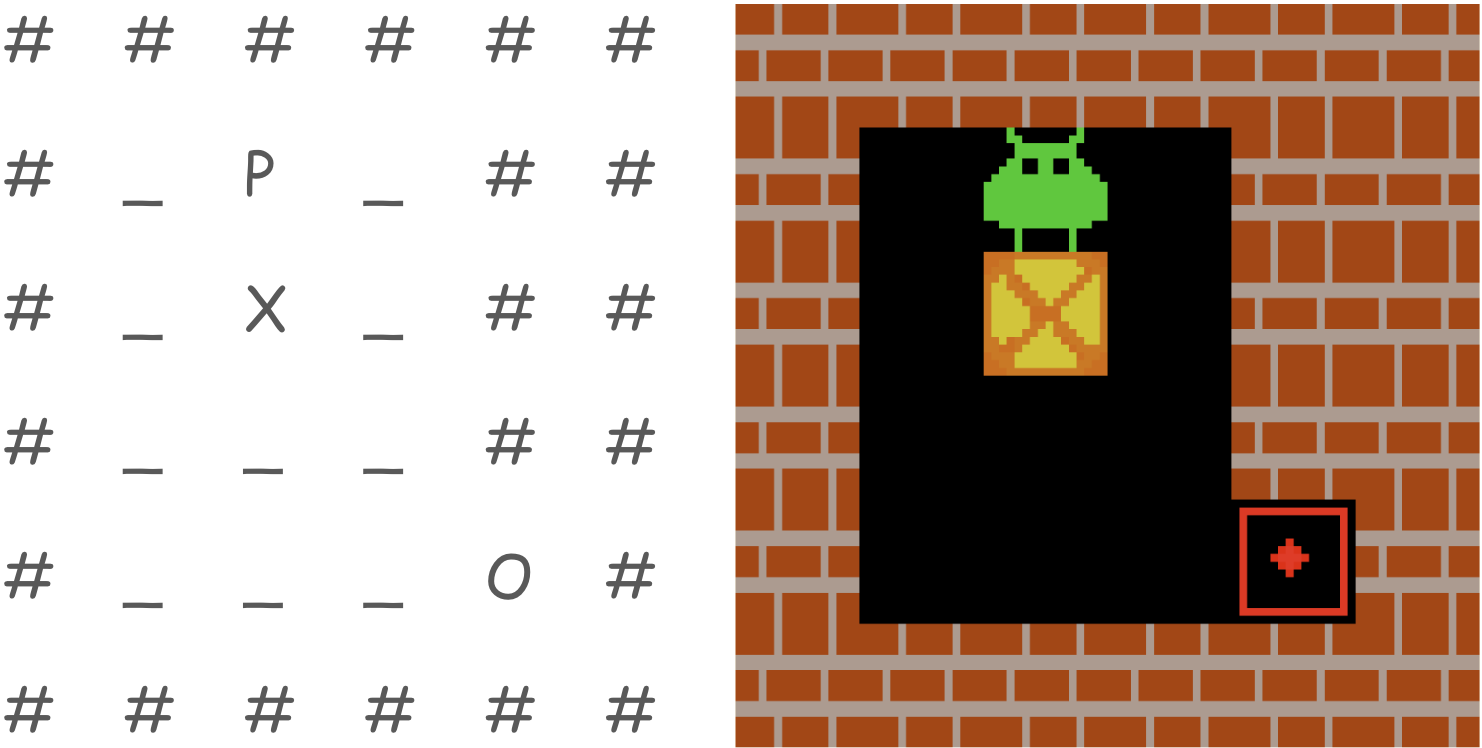
\includegraphics[width=\linewidth]{figures/sokoban_env_example.png}
%     \caption{Grid representation and rendered image of an example Sokoban Environment}
%     \label{fig:sokoban_env_example}
% \end{figure}

% \begin{figure}[H]
%     \centering
%     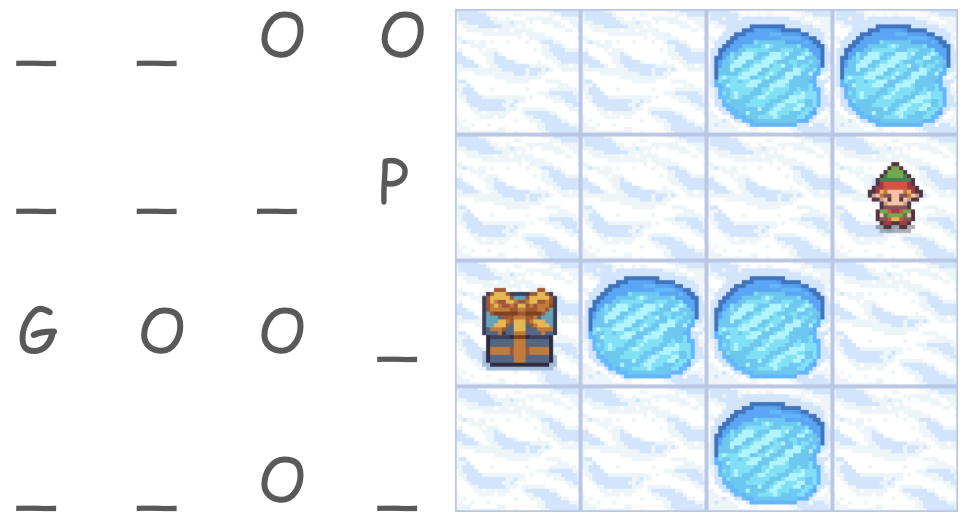
\includegraphics[width=\linewidth]{figures/frozenlake_env_example.png}
%     \caption{Grid representation and rendered image of an example FrozenLake Environment}
%     \label{fig:frozenlake_env_example}
% \end{figure}

The instruction template only consists of available actions and restrictions:

\begin{tcolorbox}[colback=gray!2, colframe=black, boxrule=0.5pt, arc=2pt, width=0.95\linewidth, title=Instruction Template]
\texttt{Your available actions are:\\
Up, Down, Left, Right\\
You can make up to 10 actions, separated by the action separator " || "
}
\end{tcolorbox}

% The environment provides state updates through different rendering modes:

% \begin{promptbox}{State Rendering Modes}
% \textbf{Available Modes:}\\
% tiny\_rgb\_array: Text-based grid representation\\
% list: Space-separated grid symbols\\
% state: Numerical state matrix\\
% rgb\_array: Visual representation as image

% \textbf{Rendering Format:}\\
% Grid cells are separated by tabs horizontally\\
% Rows are separated by newlines\\
% Each cell is padded with spaces for readability
% \end{promptbox}


\subsection{FrozenLake Environment Prompts}

The FrozenLake environment implements a grid-world navigation task where an agent must traverse a slippery frozen surface to reach a goal. Below we detail the prompt structure used for this environment.

\begin{tcolorbox}[colback=gray!2, colframe=black, boxrule=0.5pt, arc=2pt, width=0.95\linewidth, title=Model Templates]
% \textbf{Instruct Model Template:}

\texttt{<|im\_start|>system\\
\{prompt\}\\
You're a helpful assistant. You always respond by first wrapping your thoughts in <think>...</think>, then giving your answer in <answer>...</answer>. Max response length: 200 words (tokens).\\
<|im\_end|>\\
<|im\_start|>user\\
\{prompt\}\\
You are solving the FrozenLake puzzle. Forbid the whole and go to the target. You may move to the unintended direction due to the slippery ice. Example answer format: <think>To forbid the hole and go to the target, I should go left then go up.</think><answer>Left || Up</answer>\\
<|im\_end|>\\
<|im\_start|>assistant\\
<think>}

% \textbf{Base Model Template:}

% \texttt{A conversation between User and Assistant. The user asks a question, and the Assistant solves it. The assistant first thinks briefly about the reasoning process in the mind and then provides the user with the answer.\\
% User: \{prompt\}\\
% Show your work in <think> </think> tags. And return the final answer in <answer> </answer> tags, for example <think> [Thoughts] </think> <answer> 1 </answer>\\
% Assistant:\\
% <think>}
\end{tcolorbox}


% \begin{promptbox}{Task Introduction}
% You are walking on a frozen lake.

% \textbf{FrozenLake Quick Guide}\\
% Goal: Reach the goal (G).

% \textbf{Symbols:}\\
% \_ Frozen\\
% O Hole\\
% G Goal\\
% P Player

% \textbf{Rules:}\\
% Avoid falling into holes (O).\\
% Frozen tiles are slippery, you may move perpendicular to your intended direction.

% \textbf{Answers:}\\
% \texttt{<answer> Up </answer>}\\
% \texttt{<answer> Down </answer>}\\
% \texttt{<answer> Left </answer>}\\
% \texttt{<answer> Right </answer>}

% \textbf{Rewards:}\\
% Fall into hole: 0\\
% Reach goal: +1.0
% \end{promptbox}

The environment uses a grid-based representation with specific symbols for different elements:

\begin{tcolorbox}[colback=gray!2, colframe=black, boxrule=0.5pt, arc=2pt, width=0.95\linewidth, title=Grid Representation]
\texttt{
The meaning of each symbol in the state is:\\
P: player, \_: empty, O: hole, G: goal, X: player in hole, $\checkmark$: player on goal
}
\end{tcolorbox}

The instruction template only consists of available actions and restrictions:

\begin{tcolorbox}[colback=gray!2, colframe=black, boxrule=0.5pt, arc=2pt, width=0.95\linewidth, title=Instruction Template]
\texttt{Your available actions are:\\
Left, Down, Right, Up\\
You can make up to 10 actions, separated by the action separator " || "
}
\end{tcolorbox}

% The environment supports multiple rendering modes for state observation:

% \begin{promptbox}{State Rendering Modes}
% \textbf{Rendering Format:}\\
% Grid cells are separated by tabs horizontally\\
% Rows are separated by newlines\\
% Special handling for start position ('S' replaced with 'F')\\
% Player position updated dynamically in rendering
% \end{promptbox}
